\scanpage{17}
\mspage{\textcircled{3}}

\unsure{quadrilatère|quadrilatere}

\[\resizebox{\ifdim\width>\linewidth\linewidth\else\width\fi}{!}{$\displaystyle
\begin{aligned}
 &-x_1x_2y_{\deleted{\unsure{3}}1}y_{\deleted{\unsure{1}}3}
 +y_1y_2x_1x_3\\
 &\tikz[baseline=(n.base)]\node[draw,rounded corners=12pt](n){$=-x_{1}y_1(x_2y_3-y_2x_3)$};
\end{aligned}
$}\]

\noindent\rule{.6\linewidth}{.4pt}

\[\resizebox{\ifdim\width>\linewidth\linewidth\else\width\fi}{!}{$\displaystyle
\begin{aligned}
 &x_1x_2y_1\underbrace{(y_0+y_1)}_{-y_2-y_3}
 -y_1y_2x_1\underbrace{(x_0+x_1)}_{-x_2-x_3}=\\
 &=-x_1x_2y_1(y_2+y_3)+y_1y_2x_1(x_2+x_3)\\
 &=-\underline{x_1x_2y_1}y_3+\underline{y_1y_2x_1}x_3
 \quad\tikz[baseline=(n.base)]\node[draw,rounded corners=12pt](n){$=-x_1y_1(x_2y_3-y_2x_3)$};
\end{aligned}
$}\]
\[
 \boxed{\lambda_0+\lambda_1=0}
\]
\tikz[baseline=(c.base)]\node[draw,rounded corners=7pt,inner sep=2pt](c){si};\uline{ $s_3$ non aplati}
\figure{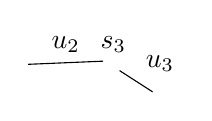
\begin{tikzpicture}
\draw (0,0)--(.95,.04) node[midway,above] {$u_2$};
\node[above] at (1.08,.02) {$s_3$};
\draw (1.16,-.08)--(1.58,-.35) node[midway,above right] {$u_3$};
\end{tikzpicture}}

\noindent\rule{\linewidth}{.4pt}

\[\resizebox{\ifdim\width>\linewidth\linewidth\else\width\fi}{!}{$\displaystyle
\begin{aligned}
 &-x_2\underset{\cdot}{x_3}\underset{\cdot}{y_3}(y_1+y_{\underset{\unsure{1}}{2}})
 +y_2\underset{\cdot}{y_3}\underset{\cdot}{x_3}(x_1+x_2)\\
 &\tikz[baseline=(n.base)]\node[draw,rounded corners=12pt](n){$=-x_3y_3(x_1y_2-y_1x_2)$};
\end{aligned}
$}\]
\[\resizebox{\ifdim\width>\linewidth\linewidth\else\width\fi}{!}{$\displaystyle
\begin{aligned}
 &x_2\underset{\cdot}{x_3}y_1\underbrace{(y_0+y_1+y_2)}_{\underset{\cdot}{-y_3}}
 -y_2\underset{\cdot}{y_3}x_1
 \underbrace{(x_0+x_{\unsure{1|4}}+x_2)}_{\underset{\cdot}{-x_3}}\\
 &\tikz[baseline=(n.base)]\node[draw,rounded corners=12pt](n){$=\unsure{+|-}x_3y_3(x_1y_2-y_1x_2)$};
 \qquad\boxed{\lambda_0+\lambda_1=0}
\end{aligned}
$}\]
\figure{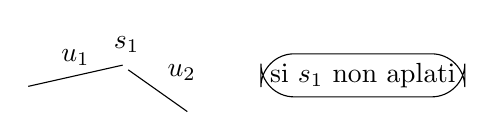
\begin{tikzpicture}
\draw (0,0)--(1.2,.27) node[midway,above] {$u_1$};
\node[above] at (1.25,.3) {$s_1$};
\draw (1.27,.21)--(2.02,-.32) node[midway,above right] {$u_2$};
\node[draw,rounded corners=12pt] at (4.25,.14) {si $s_{1}$ non aplati};
\end{tikzpicture}}

\[\resizebox{\ifdim\width>\linewidth\linewidth\else\width\fi}{!}{$\displaystyle
\begin{aligned}
 &u_0\quad u_1\quad u_2\quad u_3\\
 &u_0\wedge u_1\quad u_1\wedge u_2\quad u_2\wedge u_3\qquad
 \deleted{u_3\wedge u_0=u_3\wedge[\unsure{-}(}\\
 &\hspace{4cm}u_3\wedge u_0=-(u_0+u_1+u_2)\wedge u_0=\\
 &\hspace{5.5cm}\unsure{+|-}u_0\wedge u_1+u_0\wedge u_2
\end{aligned}
$}\]

\figure{\begin{tikzpicture}[x=.011cm,y=-.011cm]
\draw (464,2195)..controls(448,2173)and(397,2150)..(364,2104)--(416,2059);
\draw (431,2042)--(479,1992);
\draw (493,1995)..controls(516,2029)and(537,2060)..(589,2083);
\end{tikzpicture}}
\diagram{\(\begin{array}{cc}x_0&y_0\\x_1&y_1\\x_2&y_2\\x_3&y_3\end{array}\)}
% archive sheet number: 23
